\documentclass[letterpaper,12pt]{article}
\usepackage{tabularx} % extra features for tabular environment
\usepackage{amsmath}  % improve math presentation
\usepackage{float}
\usepackage{pdfpages}

\usepackage{graphicx} % takes care of graphic including machinery
\graphicspath{ {./figures/} }
\usepackage[margin=1in,letterpaper]{geometry} % decreases margins
\usepackage{cite} % takes care of citations
\usepackage[final]{hyperref} % adds hyper links inside the generated pdf file
\hypersetup{
	colorlinks=true,       % false: boxed links; true: colored links
	linkcolor=blue,        % color of internal links
	citecolor=blue,        % color of links to bibliography
	filecolor=magenta,     % color of file links
	urlcolor =blue         
}




\begin{document}

\title{Experiment 2 Preliminary Work \protect\\ Miscellaneous Opamp Circuits}
\author{Ahmet Akman 2442366 \protect\\}
\date{\today}
\maketitle
\tableofcontents
%\begin{abstract}
%abstract
%\end{abstract}

%\section{Introduction}
\section{Step 1}
In this step the independent current source circuit is investigated. The reference circuit is given in Figure 1.
\begin{figure}[H]
    \centering
    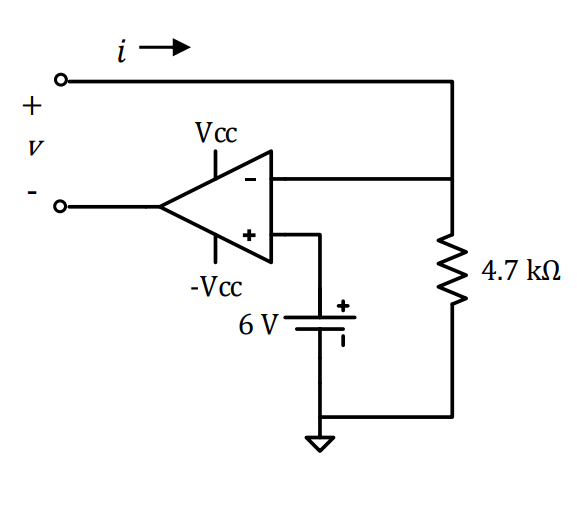
\includegraphics[width=0.65\textwidth]{1SCH.png}
\caption{Circuit schematic for the step 1}
\end{figure} 

\subsection{a)}
To obtain the i-v charactheristics, the analysis is made and given in Figure 2. The analysis also includes the part b . 
\begin{figure}[H]
    \centering
    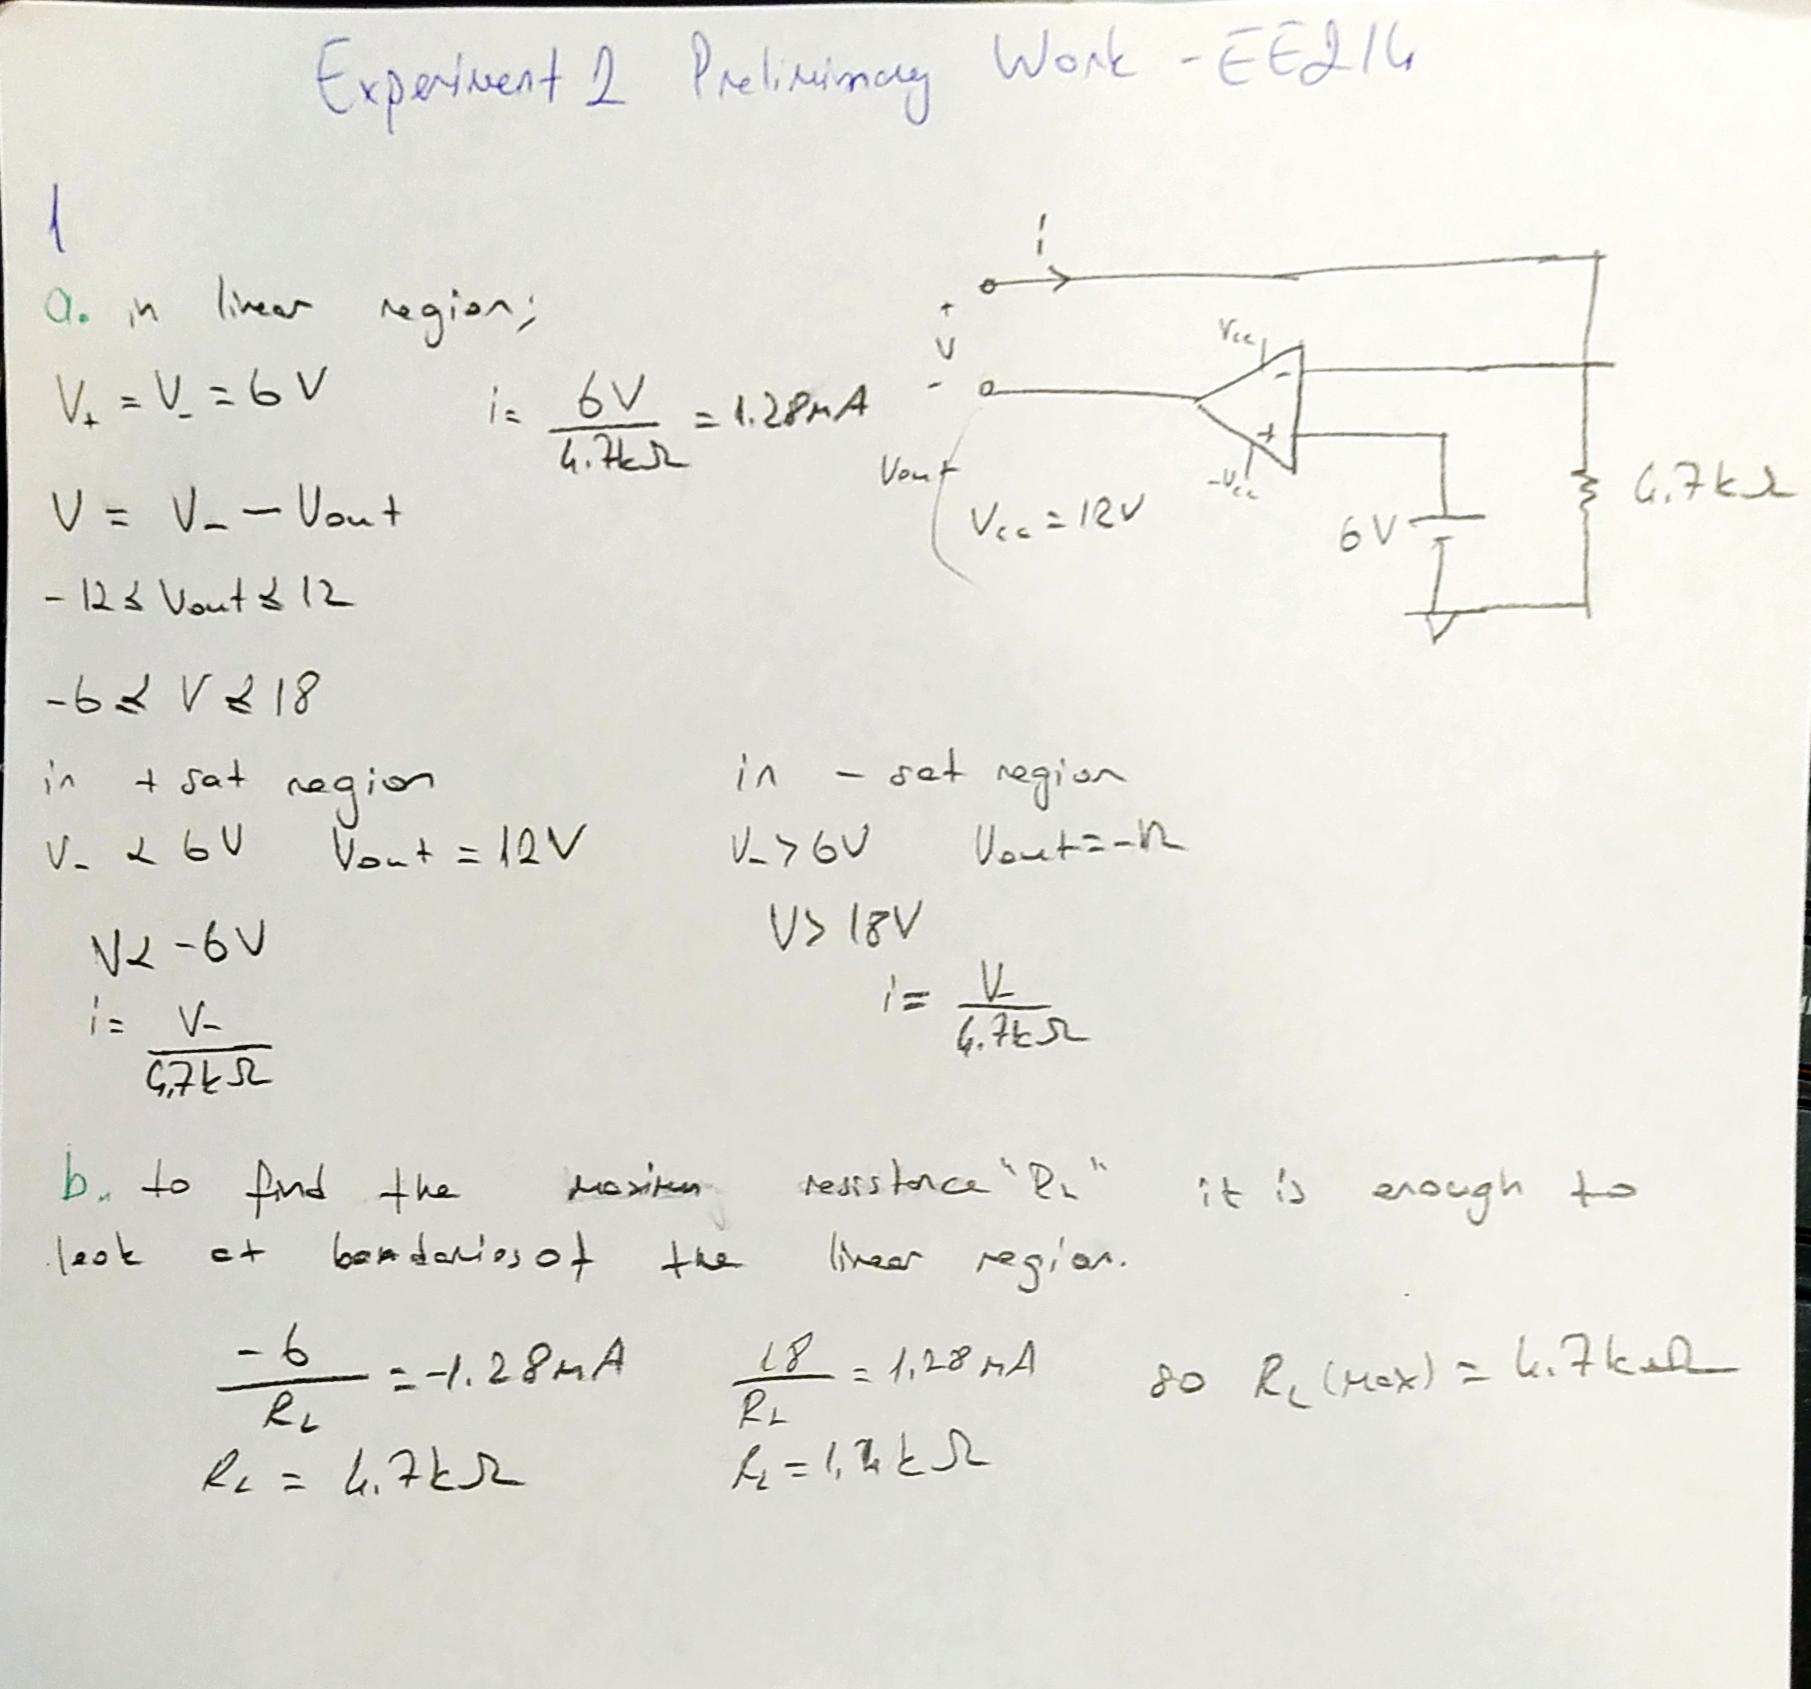
\includegraphics[width=1\textwidth]{1a.jpg}
\caption{ calculation of i-v }
\end{figure} 

\subsection{c)}
The simulation of the circuit given in Figure 1 is constructed in LTSpice environment. The schematic is given in Figure 3 .
\begin{figure}[H]
    \centering
    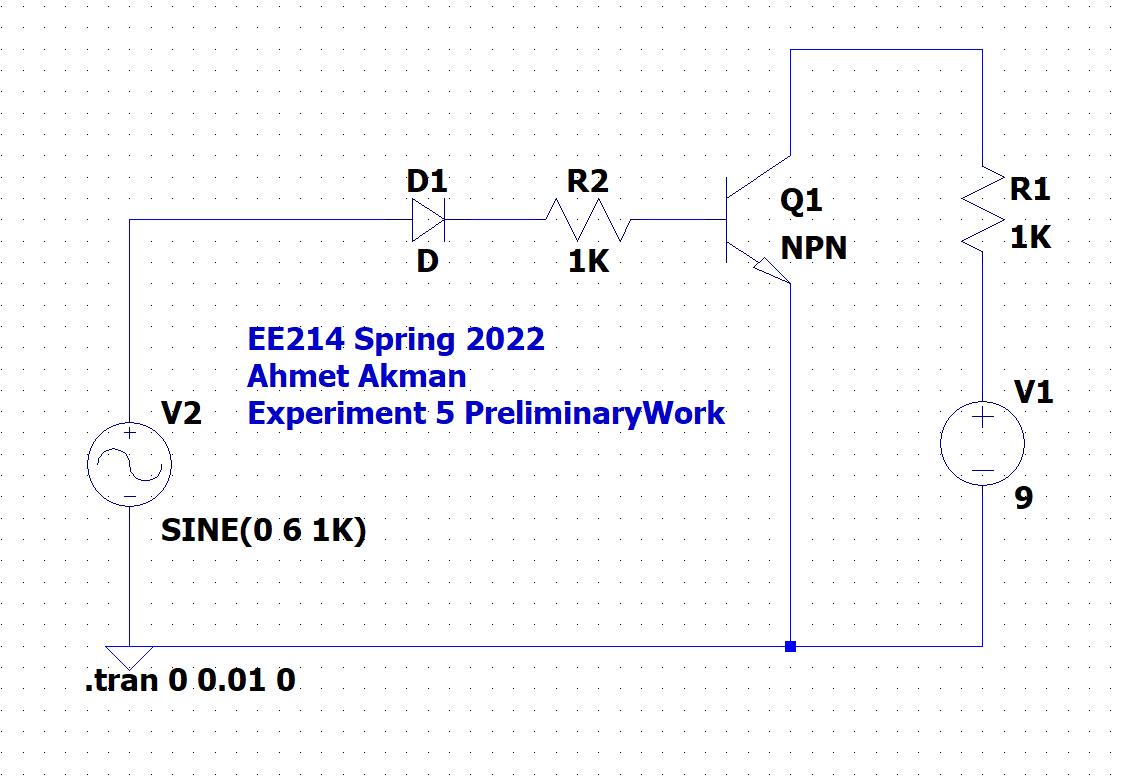
\includegraphics[width=1\textwidth]{1sim.png}
\caption{Circuit simulation schematic  for the step 1}
\end{figure} 
As a result, the plot given in Figure 4 is obtained.
\begin{figure}[H]
    \centering
    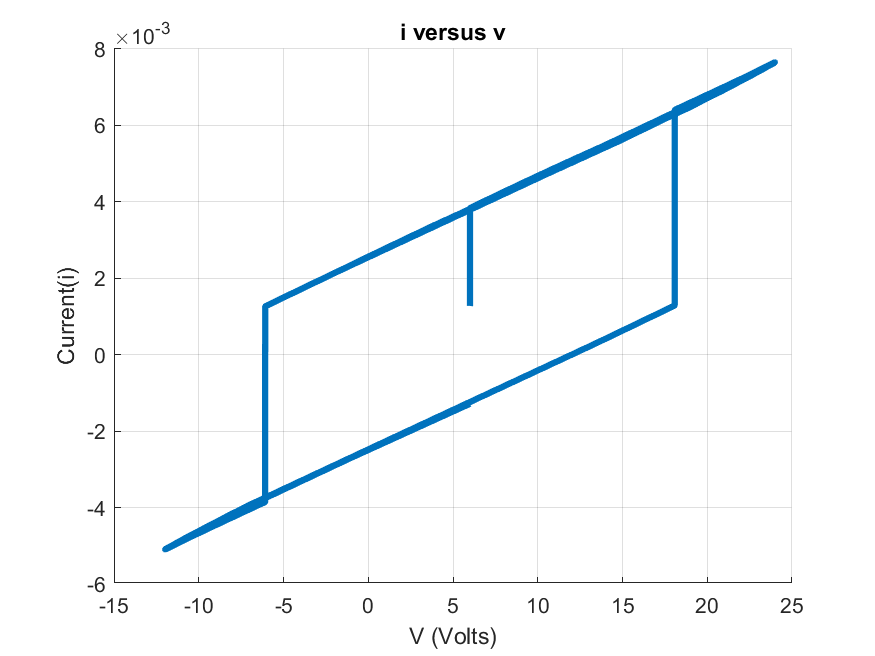
\includegraphics[width=1\textwidth]{1.png}
\caption{i versus v plot} 
\end{figure} 
So, it is again observed that in the linear region the circuit behaves like an independent current source even though it can take multiple values and seems unstable.

\section{Step 2}
The schematic is given in Figure 5 is taken as the reference .
\begin{figure}[H]
    \centering
    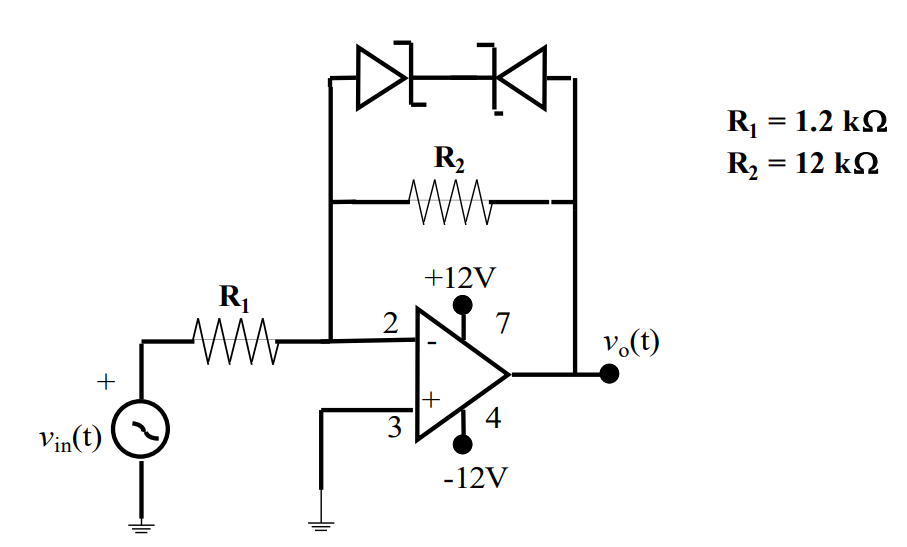
\includegraphics[width=0.65\textwidth]{2SCH.png}
\caption{Circuit schematic for the step 2}
\end{figure} 

The simulation of the circuit given in Figure 6 is constructed in LTSpice environment.
\begin{figure}[H]
    \centering
    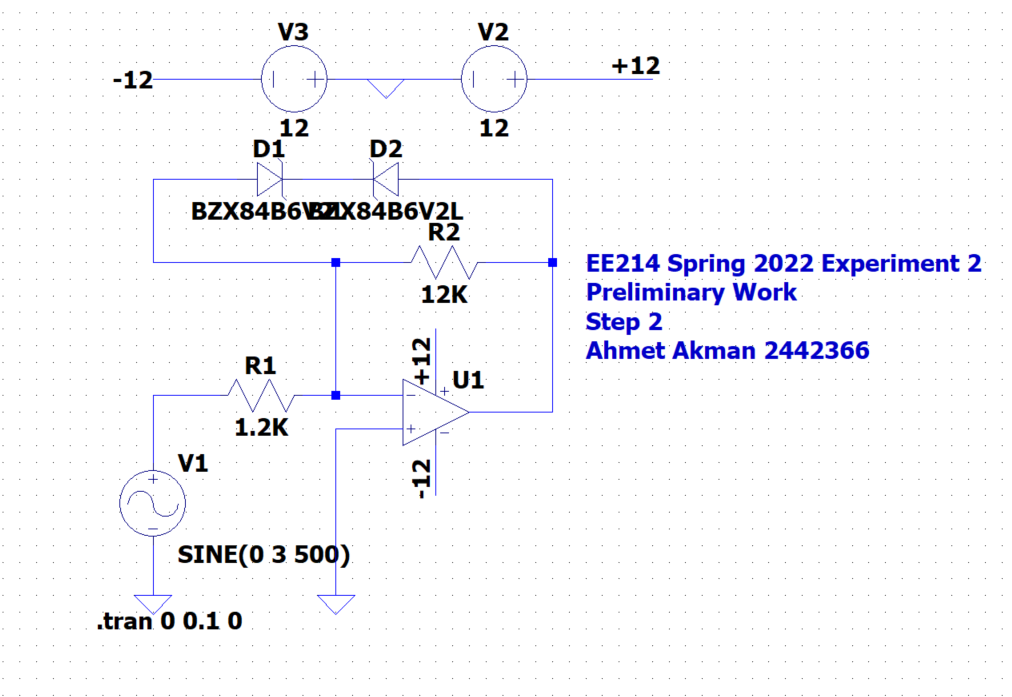
\includegraphics[width=1\textwidth]{2Sim.png}
\caption{Circuit simulation schematic  for the step 2}
\end{figure} 
As a result, the plot given in Figure 7 is obtained.
\begin{figure}[H]
    \centering
    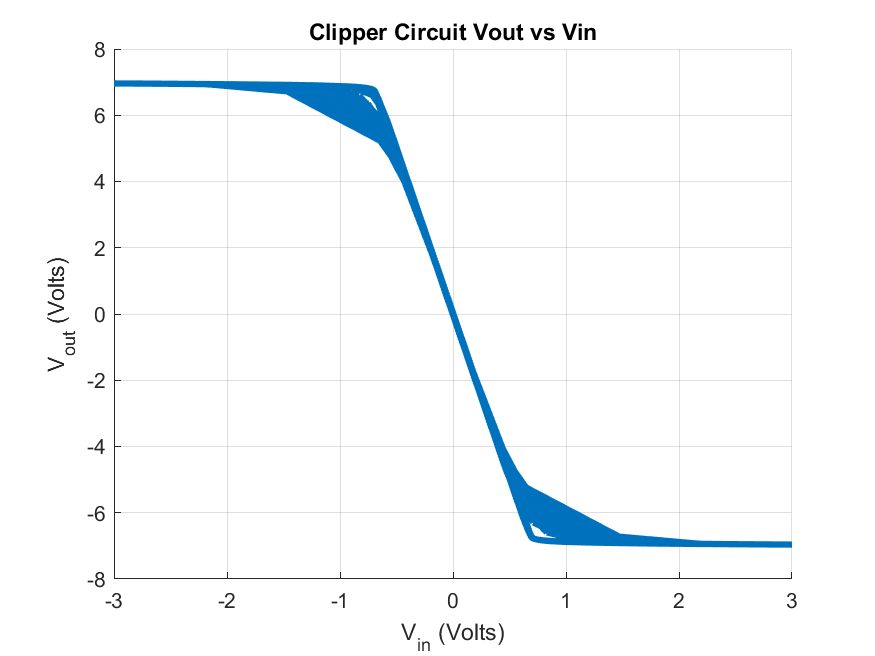
\includegraphics[width=1\textwidth]{2.png}
\caption{\(V_{in}\) and \(V_o\) versus time} 
\end{figure}  

\section{Step 3}

In this step the circuit schematic given in Figure 8 is taken as the reference.
\begin{figure}[H]
    \centering
    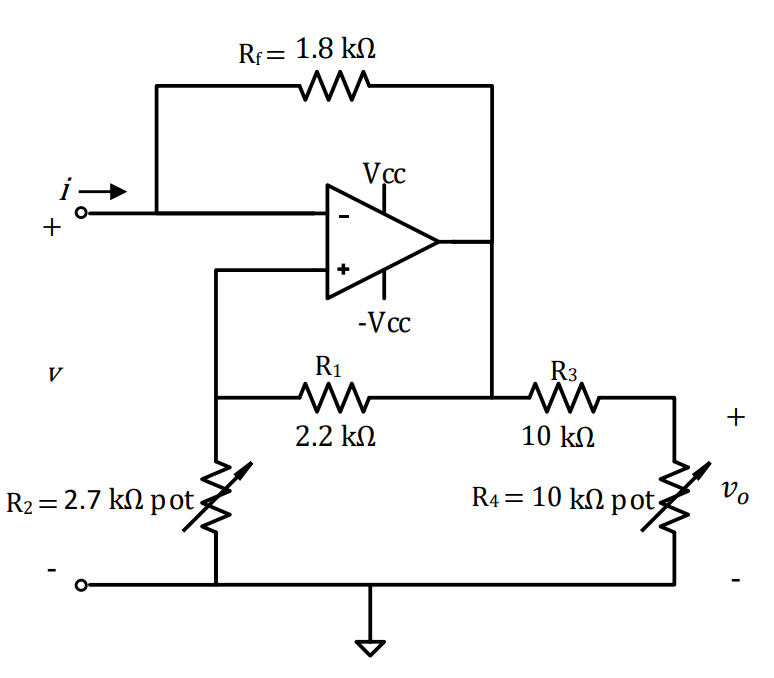
\includegraphics[width=0.65\textwidth]{3SCH.png}
\caption{Circuit schematic for the step 3}
\end{figure} 

\subsection{a)}
The calculations and skteches are made on paper as given in Figure 9 for part a.
\begin{figure}[H]
    \centering
    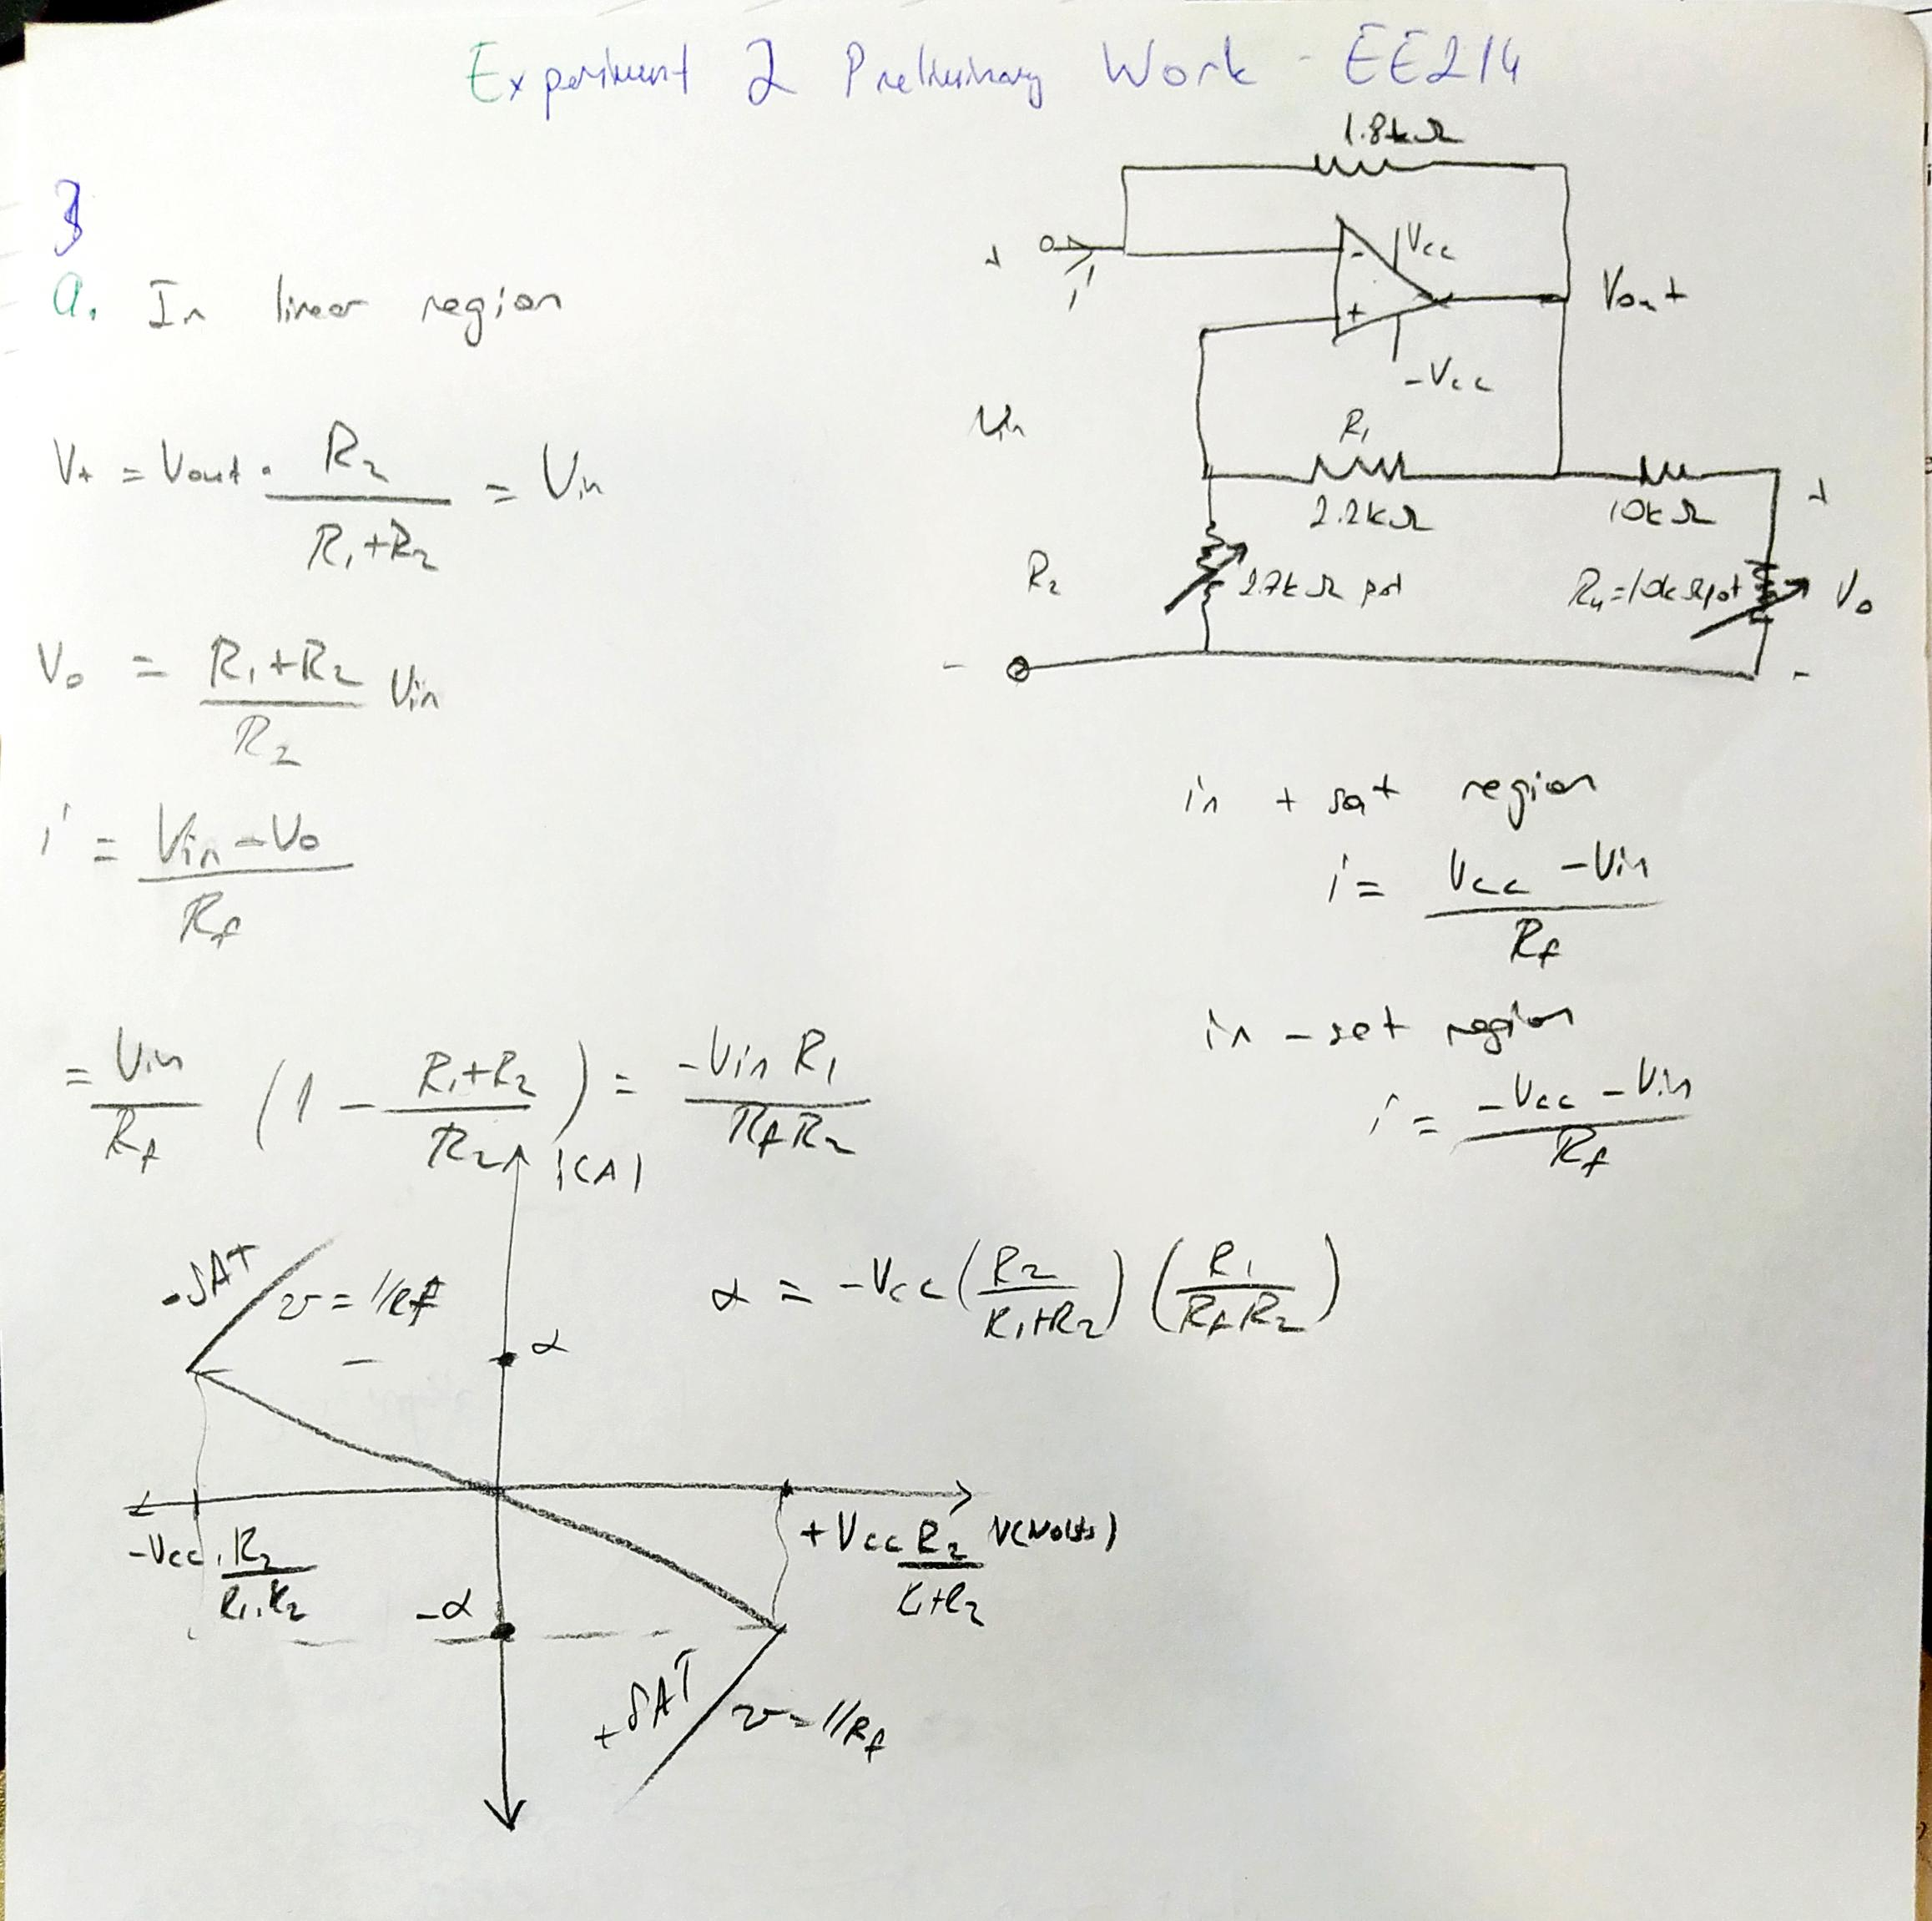
\includegraphics[width=1\textwidth]{3a.jpg}
\caption{ calculation and i-v  sketch}
\end{figure} 

\subsection{b)}
To find the factors that may effect the frequency of the resulting square wave,  in addition to the analysis made in the previous step \(V_c\) is added. The graph of the \(V_c\) shows that the capacitor is constantly charges and discharges in time. Also, the op-amp is changed between the + and - saturation regions. So the period is obtained as follows:
\[
T = -2 R_f C  ln( \frac{R_1}{R_1+R_2})    
\]
Since the frequency is the inverse of the period, it can be said that the frequency is dependent on the quantities appearing in the above expression which are \(R_f , C , R_1 \) and \(R_2\). 
Since the relation between \(V_{out}\) and \(V_o\) is simply dependent on voltage division. It is dependent on the \(V_{cc}\) , \(R_3\) and \(R_4\). 
\subsection{c)}
By looking at the equations provided in part b and the resistance values given, in order to set the frequency 500Hz, R2 should be adjusted to approximately 1.63K\(\Omega\). In order to make \(V_o\) equal to 2 Volts, (assuming the \(V{cc} is set  to 12 volts\)) the pot \(R_4 \) should be set to 2K\(\Omega\).

\subsection{d)}
The simulation of the circuit given in Figure 8 is constructed in LTSpice environment. The schematic is given in Figure 10 .
\begin{figure}[H]
    \centering
    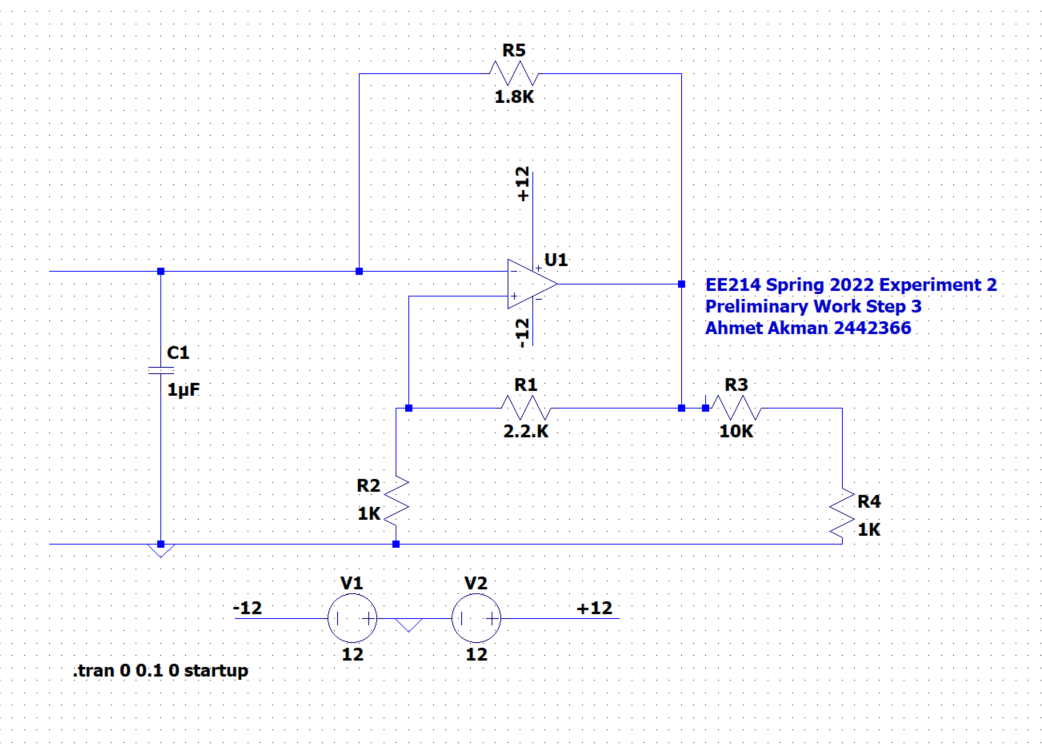
\includegraphics[width=1\textwidth]{3Sim.png}
\caption{Circuit simulation schematic  for the step 3}
\end{figure} 
As a result, the plot given in Figure 11 is obtained.
\begin{figure}[H]
    \centering
    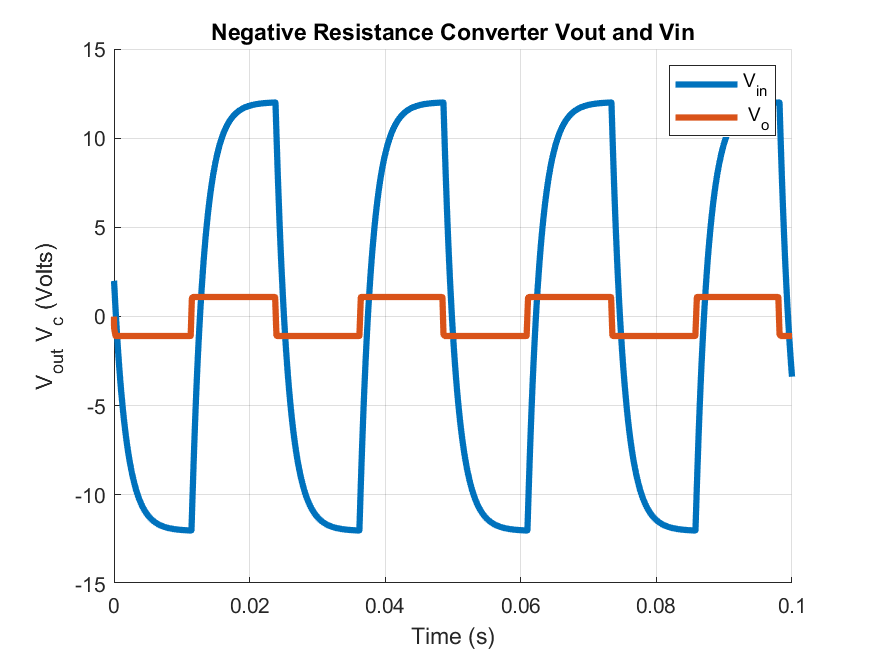
\includegraphics[width=1\textwidth]{3.png}
\caption{\(V_{in}\) and \(V_o\) versus time} 
\end{figure} 



\section{Conclusion}
In this document, three miscellaneous opamp circuits are analyzed, therefore driving point charactheristics are obtained. The simulations are made and necessary plots are obtained.  So the requirements of the preliminary work is satisfied.


\section*{Appendix A}
The results of the simulations are fetched from LTSpice and plotted in MATLAB in order to make the plots more readable and convenient.


\end{document}

%%%%%%%%%%%%%%%%%%%%%%   EXAMPLE TABLE   %%%%%%%%%%%%%%%%%%%%%%%%%%%%%%%%
\begin{table}[H]
\begin{center}
    \caption{Resistance reading by color code convention.}
    \vspace{2mm}
    \begin{tabular}{||c | c | c||} 
        \hline
        Color Order & Value & Tolerance \\ [0.5ex] 
        \hline\hline
        Brown / Black / Red / Gold & 1k\( \Omega \) & \( \% \) 5  \\ 
        \hline
        Yellow / Violet / Red / Gold & 4.7k\( \Omega \) & \( \% \) 5   \\
        \hline
        Brown / Grey / Orange / Gold & 18k\( \Omega \) & \( \% \) 5  \\ [1ex] 
        \hline
    \end{tabular}
\end{center}
\end{table}


%%%%%%%%%%%%%%%%%%%%%%   EXAMPLE IMAGE   %%%%%%%%%%%%%%%%%%%%%%%%%%%%%%%%
\begin{figure}[H]
\centering
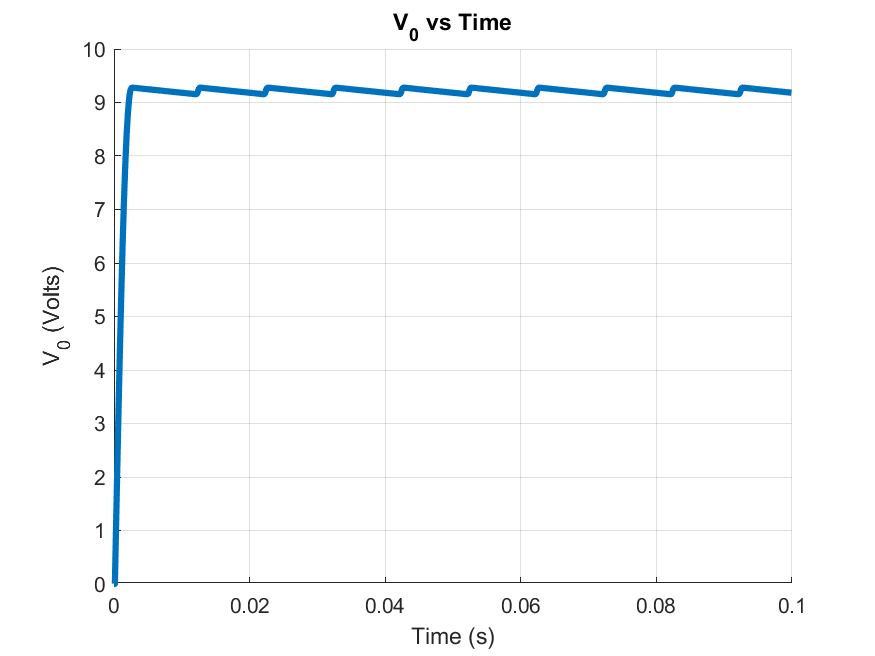
\includegraphics[width=1\textwidth]{5.png}
\caption{Circuit schematic for the step 5}
\end{figure} 

%%%%%%%%%%%%%%%%%%%%%%   EXAMPLE IMAGE FROM PDF   %%%%%%%%%%%%%%%%%%%%%%%%%%%%%%%%
\begin{figure}[H] \centering{
	\includegraphics[scale=0.25]{2a_plot.pdf}}
	\caption{Experiment 2}
\end{figure}
	